\documentclass{ximera}

\title{POI-Discontinuities Practice}
\begin{document}
\begin{abstract}
    Practice for Points of Interest - Discontinuities.
\end{abstract}
\maketitle


\begin{problem}
    Consider the following graph.
    \begin{center}
        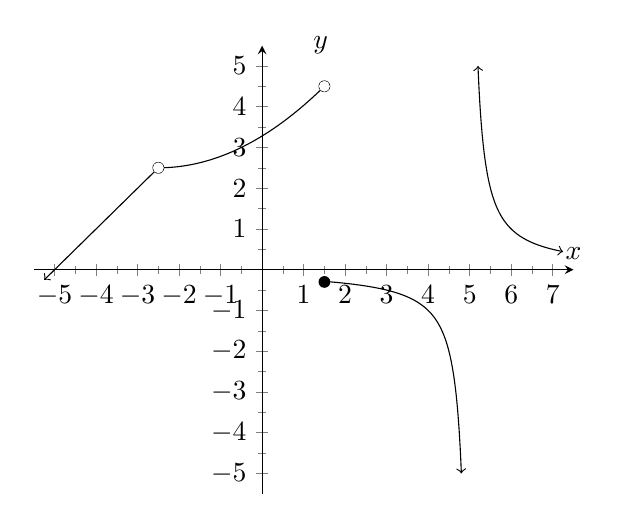
\begin{tikzpicture}
                \begin{axis}[
                    axis x line=middle, 
                    axis y line=middle, 
                    minor tick num=1, 
                    x label style={at={(axis description cs:1,0.5)},anchor=south},
                    y label style={at={(axis description cs:0.5,1)},anchor=west},
                    xlabel={$x$}, 
                    ylabel={$y$},
                    xtick={-5,-4,...,6,7}, 
                    ytick={-5,-4,...,5},
                    xmin=-5.5, 
                    xmax=7.5, 
                    ymin=-5.5, 
                    ymax=5.5
                    ]
                \addplot[<-,domain=-5.25:-2.5, samples=300]{x+5};
                \addplot[domain=-2.5:1.5, samples=300]{1/8*(x+2.5)^2+2.5};
                \addplot[->,domain=1.5:4.8, samples=300]{1/(x-5)};
                \addplot[<->,domain=5.2:7.25, samples=300]{1/(x-5)};
                \node[label={180:{}},circle,fill,inner sep=1.5pt] at (axis cs:-2.5,2.5) {};
                \node[label={180:{}},circle,fill,white,inner sep=1.4pt] at (axis cs:-2.5,2.5) {};
                \node[label={180:{}},circle,fill,inner sep=1.5pt] at (axis cs:1.5,4.5) {};
                \node[label={180:{}},circle,fill,white,inner sep=1.4pt] at (axis cs:1.5,4.5) {};
                \node[label={270:{}},circle,fill,inner sep=1.5pt] at (axis cs:1.5,-0.3) {};
                \end{axis}
        \end{tikzpicture}
    \end{center}
    
    Does the above graph have any hole discontinuities?
    \begin{multipleChoice}
        \choice[correct]{Yes}
        \choice{No}
    \end{multipleChoice}
    
    \begin{problem}
        What is the approximate $x$-value of the hole? $\answer{-2.5}$
        \begin{feedback}
            A hole is the type of discontinuity that is a single missing point in an otherwise continuous graph. This may not look like it quite right (another example of graphing being misleading, but not on purpose this time) but the $x$-value is actually $-2.5$.
        \end{feedback}
    
        \begin{problem}
            Is there a jump discontinuity?
            \begin{multipleChoice}
                \choice[correct]{Yes}
                \choice{No}
            \end{multipleChoice}
            
            \begin{problem}
                What is the approximate $x$-value of the jump discontinuity? $\answer{1.5}$
                \begin{feedback}
                    A jump discontinuity is the type of discontinuity that has a \textit{finite} vertical jump between the end points.
                \end{feedback}
                \begin{problem}
                    Is there an infinite discontinuity?
                    \begin{multipleChoice}
                        \choice[correct]{Yes}
                        \choice{No}
                    \end{multipleChoice}
                    
                    \begin{problem}
                        What is the approximate $x$-value of the infinite discontinuity? $\answer{5}$
                        \begin{feedback}
                            An infinite discontinuity is the type of discontinuity that has a vertical asymptote.
                        \end{feedback}
                    \end{problem}
                \end{problem}
            \end{problem}
        \end{problem}
    \end{problem}
\end{problem}


\end{document}